% !TEX root = main.tex
\documentclass[twocolumn]{article}
\usepackage[a4paper,margin=1in]{geometry} 
\usepackage{lmodern}
\usepackage{setspace}
\usepackage{mathptmx}
\usepackage{algorithm}
\usepackage{algpseudocode}
\usepackage{amsmath}
\usepackage{booktabs}
\usepackage{arydshln}
\usepackage{float}
\usepackage{cite}
\usepackage{multirow}
\usepackage{graphicx}
\usepackage{url}
\usepackage{import}

\title{\huge \textbf{Words That Matter:\\ Vocabulary Pruning in ModernBERT}}
\author{Wout De Rijck, Dr. Ir. Karel D'Oosterlinck, \\ Prof. Dr. Ir. Thomas Demeester, Prof. Dr. Ir. Chris Develder}
\date{} % No date

\begin{document}
\maketitle
% Motivation / Context (1–2 sentences):
% Start with the why. What's the broader problem or challenge? Why is this area important right now (e.g., limitations of current LLMs, safety, interpretability, efficiency)?

% Gap / Problem Statement:
% What specific problem or limitation does your paper address? This sets the stage for your contribution. It should hint at a shortcoming in current approaches without being overly critical.

% Your Approach / Contribution:
% What did you do? This is the heart of the abstract. It could be:

% a new method or model

% a novel dataset or benchmark

% a unique analysis or framework

% an improvement on performance, interpretability, etc.

\begin{abstract}
Large language models like ModernBERT deliver impressive performance but face a critical deployment challenge: their substantial computational and memory demands restrict their use in resource-constrained environments. While various pruning techniques exist to address this bottleneck, most require expensive post-pruning fine-tuning—creating a paradoxical situation where model optimization itself demands significant resources. This paper introduces a novel vocabulary pruning approach for ModernBERT that eliminates the need for post-pruning recovery fine-tuning, delivering superior efficiency particularly at smaller pruning ratios (5-20\%). The proposed technique specifically targets the embedding layer—which constitutes 25.95\% of the model's parameters but remains surprisingly underexplored in compression research—through systematic token importance analysis based on TF-IDF with specialized out-of-vocabulary (OOV) token handling. Experiments on the GLUE benchmark demonstrate that vocabulary pruning alone achieves 20-23\% parameter reduction while maintaining 99.2\% of the original performance, outperforming encoder-based pruning methods at these ratios. 
Benchmark measurements confirm practical benefits: 20\% reduction in storage size, about 15\% reduction in GPU memory, and no impact on inference time. This work establishes an efficient pathway for creating lightweight, task-specific transformer models through offline pre-fine-tuning optimizations rather than computationally expensive retraining.
\end{abstract}

% Key Results:
% Give a quick summary of your main findings or improvements—include metrics or comparisons if possible, but keep it digestible.

% Implications / Why It Matters:
% What's the takeaway? How might this move the field forward, or be used by other researchers or practitioners?

% Tone and Tease:
% While all of the above should be there, the language should still invite curiosity. Think clear, precise, but also hook-y—like:
% "We show that…", "Surprisingly, we find…", "This reveals a new direction for…"

\section{Introduction}

Language models like ModernBERT have revolutionized natural language processing, achieving unprecedented performance across virtually every core NLP task—from sentiment analysis and natural language inference to question answering and summarization. However, this remarkable progress comes with a significant cost: a state-of-the-art model requiring multiple gigabytes of memory simply cannot run on the billions of smartphones, IoT devices, and edge computing platforms that could benefit most from NLP capabilities. This deployment gap—between what's technically possible in research environments and what's practically deployable in the real world—represents one of the most pressing challenges in making advanced AI accessible. The success of these models stems from massive embedding layers and deep stacks of self-attention and feed-forward blocks, which together learn extraordinarily rich, contextualized token representations. Yet this very scale makes them difficult to deploy: memory footprints measured in multiple gigabytes, inference latencies unsuited to on-device or real-time use, and the sheer cost of fine-tuning or retraining pruned variants can all stand in the way of practical adoption.
\\ \\
Pruning—selectively removing parameters deemed non-essential—has emerged as one of the most promising paths to slim down these models. To date, however, the majority of work has focused on sparsifying or structurally pruning the encoder layers: zeroing out small weights in feed-forward networks, dropping entire attention heads, or even omitting full transformer blocks during inference. While these methods can yield substantial compression, they often require additional fine-tuning to recover lost accuracy, and they overlook a particularly "heavy" component of transformer architectures: the embedding layer. This tunnel vision in pruning research represents a missed opportunity for significant efficiency gains.
\\ \\
In BERT-style models, the token embedding matrix alone can account for 25.95\% of all parameters in ModernBERT, yet vocabulary pruning remains comparatively underexplored. Simple heuristics—such as keeping only tokens observed in a downstream training corpus—provide a strong starting point and can achieve substantial size reductions with minimal performance impact. However, as the experiments in this paper demonstrate, these approaches don't fully capture semantic importance, miss opportunities to optimize token relationships, and often lack principled strategies for handling out-of-vocabulary tokens. While effective, they leave room for more sophisticated techniques that can push compression limits further while maintaining semantic integrity. This paper advances embedding-level pruning from a useful baseline to a central, integral component of model compression pipelines.
\\ \\
This paper presents a vocabulary pruning approach for ModernBERT~\cite{modernbert2023} that operates as a pre-fine-tuning optimization step and directly addresses these gaps. The method proceeds in two complementary stages. First, a task-specific token importance analysis using TF-IDF scores---balancing how often a token appears in the target dataset against its informativeness across the corpus---identifies and retains only the most critical subword embeddings. Second, rather than relegating all pruned tokens to a generic [UNK] index, semantic clustering over the removed embeddings maps each out-of-vocabulary token to its nearest cluster representative. This preserves nuanced semantic relationships without expanding the model's vocabulary size.
\\ \\
Because this pruning pipeline operates purely as a pre-fine-tuning optimization step and introduces no additional gradient updates, it can be applied to any pre-trained transformer with minimal overhead. Moreover, it dovetails seamlessly with existing encoder-layer pruning techniques---such as LoSparse's~\cite{losparse2023} combined low-rank plus sparse factorization---enabling an end-to-end compression strategy that tackles both embeddings and intermediate representations.
\\ \\
Validation on the GLUE benchmark suite~\cite{wang2018glue} shows that ModernBERT's embedding matrix can be reduced by up to 77.34\% (translating to a 20\% total parameter reduction) while incurring less than 1\% average degradation in downstream accuracy. The approach demonstrates superior performance compared to encoder-layer pruning techniques at lower pruning ratios (5-20\%), with practical benefits including 20\% reduction in storage size and 14.83\% reduction in GPU memory requirements. When combined with LoSparse encoder pruning for more aggressive compression, overall parameter reduction exceeds 35\% with still under 2\% performance loss---demonstrating that vocabulary and encoder pruning are both necessary and synergistic for building lightweight, high-performance transformer models.
\\ \\
In summary, the contributions of this paper are:

\begin{itemize}
    \item A vocabulary pruning methodology that operates as a pre-fine-tuning optimization step, eliminating the need for post-pruning recovery fine-tuning typically associated with model compression.
    
    \item A systematic comparison of token importance estimation techniques, revealing that TF-IDF with OOV handling provides the most robust performance across diverse NLP tasks.
    
    \item Empirical evidence that vocabulary pruning outperforms encoder-based pruning at lower pruning ratios (5-20\%), offering a more efficient pathway for moderate model compression.
    
    \item Practical deployment benefits including 20\% reduction in storage size and 14.83\% reduction in GPU memory with no inference time penalty.
\end{itemize}
By placing vocabulary pruning on equal footing with encoder-layer sparsification, Words That Matter opens a practical pathway to more compact, efficient, and deployable transformer models---bringing state-of-the-art NLP within reach of resource-constrained environments.

\section{Related work}
Model compression techniques enhance the efficiency of large language models (LLMs) by reducing their size and computational requirements. Most modern LLM compression approaches operate under post-training settings, eliminating the need for resource-intensive retraining. Model compression strategies for LLMs can be categorized into four primary methods:

\begin{enumerate}
    \item Quantization: Reduces the numerical precision of model weights, decreasing memory footprint while maintaining reasonable performance.
    
    \item Parameter pruning: Eliminates redundant or less important connections and neurons to create sparser models with fewer parameters.
    
    \item Low-rank approximation: Decomposes weight matrices into lower-dimensional representations that capture essential information while requiring fewer parameters.
    
    \item Knowledge distillation: Transfers knowledge from larger teacher models to smaller student models, enabling competitive performance with reduced architecture size.
\end{enumerate}
These approaches are complementary and can be combined to achieve optimal compression from different perspectives. 
This work focuses on pruning techniques to reduce model size while preserving performance.
For ModernBERT, an encoder-only model, this research examines specific pruning methods for encoder layers and separate techniques for the embedding matrix.

\subsection{Vocabulary Pruning Techniques}

Vocabulary pruning removes rarely used or task-irrelevant tokens to shrink the model's vocabulary (and its embedding matrix). Early work by Abdaoui et al.~\cite{abdaoui2020load} showed that most parameters of multilingual BERT lie in the embedding layer, so trimming unused language tokens can dramatically cut size. In "Load What You Need," they drop languages from mBERT's vocabulary and obtain up to a 45\% reduction in total parameters with comparable accuracy on XNLI.
\\ \\
More recently, Nair et al.~\cite{nair2023blade} proposed \textbf{BLADE}: they prune a bilingual mBERT vocabulary to include only tokens from the query and document languages for cross-lingual IR, then apply a small intermediate pretraining step. This pruned model (keeping only needed embeddings) reduced parameters by $\sim$36.5\% versus full mBERT and sped up training by $\sim$30\% and inference by $\sim$55\%, with minimal loss in retrieval quality.
\\ \\
Dorkin et al.~\cite{dorkin2025estonian} also evaluated pruning for an Estonian adaptation: pruning all tokens unused by Estonian led to no degradation on NER, whereas retraining a new tokenizer hurt performance. These studies consistently find that deleting infrequently seen subwords yields large size savings with little accuracy drop.
\\ \\
TextPruner by Shen et al.~\cite{shen2022textpruner} automates vocabulary pruning: it scans a corpus and removes any tokenizer token not present in the text, deleting its row in the embedding matrix. This simple "drop unused tokens" mode can cut model size and speed up training/inference on that domain.
\\ \\
In sparse-retrieval models like SPLADE, vocabulary pruning is implicit. SPLADE-X~\cite{formal2023spladex} (multi-lingual) restricted output to query-language tokens only, effectively pruning all other vocab. BLADE extends this idea by explicitly building a pruned bilingual model with only the union of query and document subwords, discarding other embeddings entirely.
\\ \\
Across tasks and languages, pruned-vocabulary models often match full models. For example, after pruning, Nair et al.~\cite{nair2023blade} report retrieval effectiveness on par with larger baselines, while achieving much faster indexing. Dorkin et al.~\cite{dorkin2025estonian} explicitly note "vocabulary pruning has no observable negative effect on the downstream task" (Estonian NER). These findings suggest vocabulary pruning is an effective way to tailor large models to specific domains or languages.

\subsection{Embedding-Layer Pruning and Compression}

Pruning the embedding layer often means removing or compressing rows (token vectors) to shrink this heavy component. \textbf{Partial Embedding Matrix Adaptation (PEMA)} by Bousquet et al.~\cite{bousquet2023pema} is one systematic approach: they first note that fine-tuning datasets typically use only a small fraction of the full vocabulary. PEMA therefore builds a partial embedding matrix containing only tokens seen in the task data, training on that smaller matrix. This saves GPU memory during fine-tuning without altering task accuracy. After fine-tuning, the updated embeddings are merged back into the full matrix so the model structure remains unchanged. Experiments show large memory reductions: e.g., BERT$_{\text{BASE}}$'s embedding matrix can shrink by $\sim$47\% on average (and RoBERTa by $\sim$52\%) when only task-relevant tokens are kept. Multilingual models see even more savings (mBERT $\sim$44\% embedding reduction, XLM-R $\sim$64\%) because their vocabularies are huge. Crucially, PEMA reports no drop in downstream performance, making it a practical way to prune embeddings during training.
\\ \\
Another approach is \textbf{embedding compression} via factorization or hashing. Wang et al.~\cite{wang2023lighttoken} propose \textbf{LightToken}, which compresses the entire embedding matrix using low-rank SVD plus a binary residual autoencoder. They note token embeddings are highly redundant (the embedding takes $\sim$21--31\% of BERT/RoBERTa's size). LightToken first applies a rank-$k$ SVD to capture most variation, then learns compact hash codes to reconstruct the residual. In experiments on GLUE, LightToken achieves very high compression (e.g., 25$\times$ smaller embeddings) while preserving accuracy. For BERT$_{\text{BASE}}$, a 25$\times$ embedding compression yields an average GLUE score of 82.9 (baseline 83.0).
\\ \\
These methods show that even structured low-rank or quantized pruning of embeddings can yield massive space savings with minimal impact on performance.
\\ \\
Overall, embedding-layer pruning techniques exploit the fact that many token vectors (especially for rare subwords) contribute little to end-task accuracy. By either dropping unused rows (PEMA/TextPruner) or factoring and quantizing embeddings (LightToken), these methods reduce the $\sim$25--50\% of model parameters in the embedding matrix, enabling lighter models in practice.

\subsection{Encoder-Layer Pruning (Auxiliary Methods)}
Although this paper focuses on vocab/embedding pruning, many complementary pruning methods work at the encoder layers. A classic example is \textbf{attention-head pruning}: Michel et al.~\cite{michel2019sixteen} discovered that a large percentage of attention heads can be removed at test time without significantly impacting performance. Voita et al.~\cite{voita2019analyzing} likewise pruned 38 of 48 encoder heads in an NMT transformer (removing $\sim$79\% of heads) with only a 0.15 BLEU loss.
\\ \\
In practice, toolkit frameworks (like TextPruner) often support head and FFN pruning alongside vocab pruning. Other methods include \textit{movement pruning}~\cite{sanh2020movement} that gradually zeros out small weights during fine-tuning, or \textit{LayerDrop}~\cite{fan2020layerdrop} which stochastically drops whole layers during training.

\section{Method}

The proposed hybrid vocabulary pruning method for ModernBERT targets the embedding layer, which constitutes approximately 25\% of the model's parameters. This approach is based on the observation that tokens in a vocabulary have varying importance for downstream tasks, and that certain tokens can be selectively removed with minimal impact on performance. The method primarily consists of two main components: token importance analysis and selective pruning, with an optional third component: semantic clustering for out-of-vocabulary (OOV) tokens that can further enhance performance in some cases.

\subsection{Pre-Fine-Tuning Pruning Procedure}
In contrast to methods that require resource-intensive post-pruning fine-tuning, the proposed vocabulary pruning approach operates as a pre-fine-tuning offline optimization step in the model adaptation pipeline. The standard workflow for adapting ModernBERT to a downstream task involves taking the pre-trained base model and fine-tuning it directly on the task data. This research modifies this workflow as follows:

\begin{enumerate}
    \item Task data analysis: The downstream task dataset is processed to extract token statistics.
    \item Token importance calculation: Based on the analysis, tokens are ranked by their importance using one of several methods (frequency, TF-IDF, attention patterns, etc.).
    \item Vocabulary pruning: The embedding layer is pruned by removing less important tokens according to the calculated rankings.
    \item Optional OOV handling: For pruned tokens, semantic clustering may be applied to create mappings to representative tokens.
    \item Model fine-tuning: The pruned model is then fine-tuned on the downstream task using standard procedures.
\end{enumerate}
All pruning techniques follow these common steps:
\begin{enumerate}
    \item Always preserve special tokens ([CLS], [SEP], [PAD], etc.) regardless of their importance scores
    \item Calculate token importance using the technique-specific method
    \item Sort tokens by their importance scores in descending order
    \item Keep the top $(100-p)\%$ highest-scoring tokens, where $p$ is the pruning percentage
    \item Create a reduced embedding matrix using only the retained tokens
\end{enumerate}
This approach front-loads the pruning work to the pre-fine-tuning phase, meaning the actual fine-tuning process remains unchanged and operates on a model that already has a reduced parameter count. The resulting pruned model maintains its standard inference pipeline while benefiting from reduced memory requirements.
\\ \\
The high-level vocabulary pruning procedure, combining importance-based token pruning with optional semantic clustering for OOV token handling, is formalized in Algorithm~\ref{alg:hybrid_pruning}.

\begin{algorithm}[H]
\caption{Vocabulary Pruning Procedure}
\label{alg:hybrid_pruning}
\begin{algorithmic}[1]
\footnotesize
\Require Pre-trained model $M$ with vocabulary $V_{orig}$, task dataset $D$, pruning ratio $p$
\Ensure Pruned model $M'$ with reduced vocabulary

\Function{ExtractTaskVocabulary}{$D, V_{orig}$}
    \State $V_{task} \gets $ unique tokens in dataset $D$
    \State $V_{special} \gets $ special tokens from $V_{orig}$ (e.g., [CLS], [SEP])
    \State \Return $V_{special} \cup V_{task}$ \Comment{Initial vocabulary reduction}
\EndFunction

\Function{RankByImportance}{$V, D$}
    \State Calculate importance scores for tokens in $V$ using selected method
    \State Sort $V$ by descending importance score
    \State \Return sorted token list
\EndFunction

\Function{PruneVocabulary}{$V_{ranked}, p, M$}
    \State $k \gets \lfloor |V_{ranked}| \times (1 - p) \rfloor$ \Comment{Number of tokens to keep}
    \State $V_{keep} \gets $ first $k$ tokens from $V_{ranked}$
    \State $V_{prune} \gets V_{ranked} \setminus V_{keep}$ \Comment{Tokens to be pruned}
    
    \If{using OOV handling}
        \State Create mapping from pruned tokens $V_{prune}$ to appropriate representatives
        \State \Return $V_{keep}$, mapping
    \Else
        \State \Return $V_{keep}$, null
    \EndIf
\EndFunction

\Function{CreateReducedModel}{$M, V_{keep}, mapping$}
    \State Extract embeddings for tokens in $V_{keep}$ from $M$
    \State Create reduced embedding matrix $E'$
    \State Update model with reduced embedding layer using $E'$
    \If{mapping is not null}
        \State Store mapping for OOV token handling during inference
    \EndIf
    \State \Return updated model
\EndFunction

\State // Main procedure
\State $V_{base} \gets $ \Call{ExtractTaskVocabulary}{$D, V_{orig}$}
\State $V_{ranked} \gets $ \Call{RankByImportance}{$V_{base}, D$}
\State $V_{keep}$, mapping $\gets $ \Call{PruneVocabulary}{$V_{ranked}, p, M$}
\State $M' \gets $ \Call{CreateReducedModel}{$M, V_{keep}$, mapping}

\State \Return $M'$ \Comment{Model ready for fine-tuning}
\end{algorithmic}
\end{algorithm}

\subsection{Token Importance Analysis}
A critical challenge in vocabulary pruning is determining which tokens to retain and which to remove. This research explores and compares several token importance estimation techniques, each with distinct theoretical foundations and practical implications for model performance. These approaches range from simple statistical methods to complex semantic analysis.

\subsubsection{Random Selection}
Tokens are pruned randomly without consideration for importance, serving as a baseline approach. In this method, tokens are selected for removal using uniform random sampling from the full vocabulary.

\subsubsection{Clustering-Based}
This approach employs agglomerative hierarchical clustering on the embedding space to group tokens with similar semantic properties. The algorithm works as follows:

\begin{enumerate}
    \item Each token's embedding vector is normalized to unit length (magnitude of 1), allowing the algorithm to compare tokens based solely on their semantic direction rather than magnitude.
    \item Agglomerative clustering begins with each token as its own cluster, then iteratively merges the closest pairs of clusters.
    \item The merging process uses average linkage, where the distance between clusters is the average distance between all pairs of embeddings across the two clusters.
    \item The algorithm stops when the target number of clusters is reached (determined by the pruning percentage).
    \item For each resulting cluster, the token closest to the centroid is identified and retained as the representative.
    \item All other tokens in the cluster are pruned from the vocabulary.
\end{enumerate}
This method preserves semantic diversity across the vocabulary while reducing redundancy. By selecting representatives closest to cluster centroids, the approach ensures that the preserved tokens maximize coverage of the semantic space. The clustering leverages the property that tokens with embeddings pointing in similar directions (high cosine similarity) tend to have similar semantic meanings, allowing one representative token to effectively substitute for multiple semantically related tokens.

\subsubsection{Frequency-Based}
Tokens are ranked by their frequency in the target dataset, with least frequently used tokens pruned first. This approach operates on the principle that rarely used tokens contribute less to model performance. The technique-specific algorithm steps are:

\begin{enumerate}
    \item Count occurrences of each token in the task-specific dataset
    \item Sort tokens by frequency (most common first)
\end{enumerate}
\subsubsection{Attention-Based}
This method leverages the attention mechanism of transformer models to identify important tokens. The key insight is that tokens receiving higher attention during inference are those the model relies on most heavily when making predictions, providing a direct measure of token importance from the model's perspective. Unlike frequency-based approaches that simply count occurrences, attention-based pruning preserves tokens that meaningfully contribute to the model's decision-making process.
\\ \\
As an illustrative example, the important tokens identified in the SST-2 dataset differ markedly between methods. Frequency-based approaches naturally prioritize common words like articles and prepositions, while attention-based analysis highlights sentiment-laden terms that are semantically relevant to the classification task.
\begin{figure*}[t]
\centering
\begin{minipage}{0.48\textwidth}
  \centering
  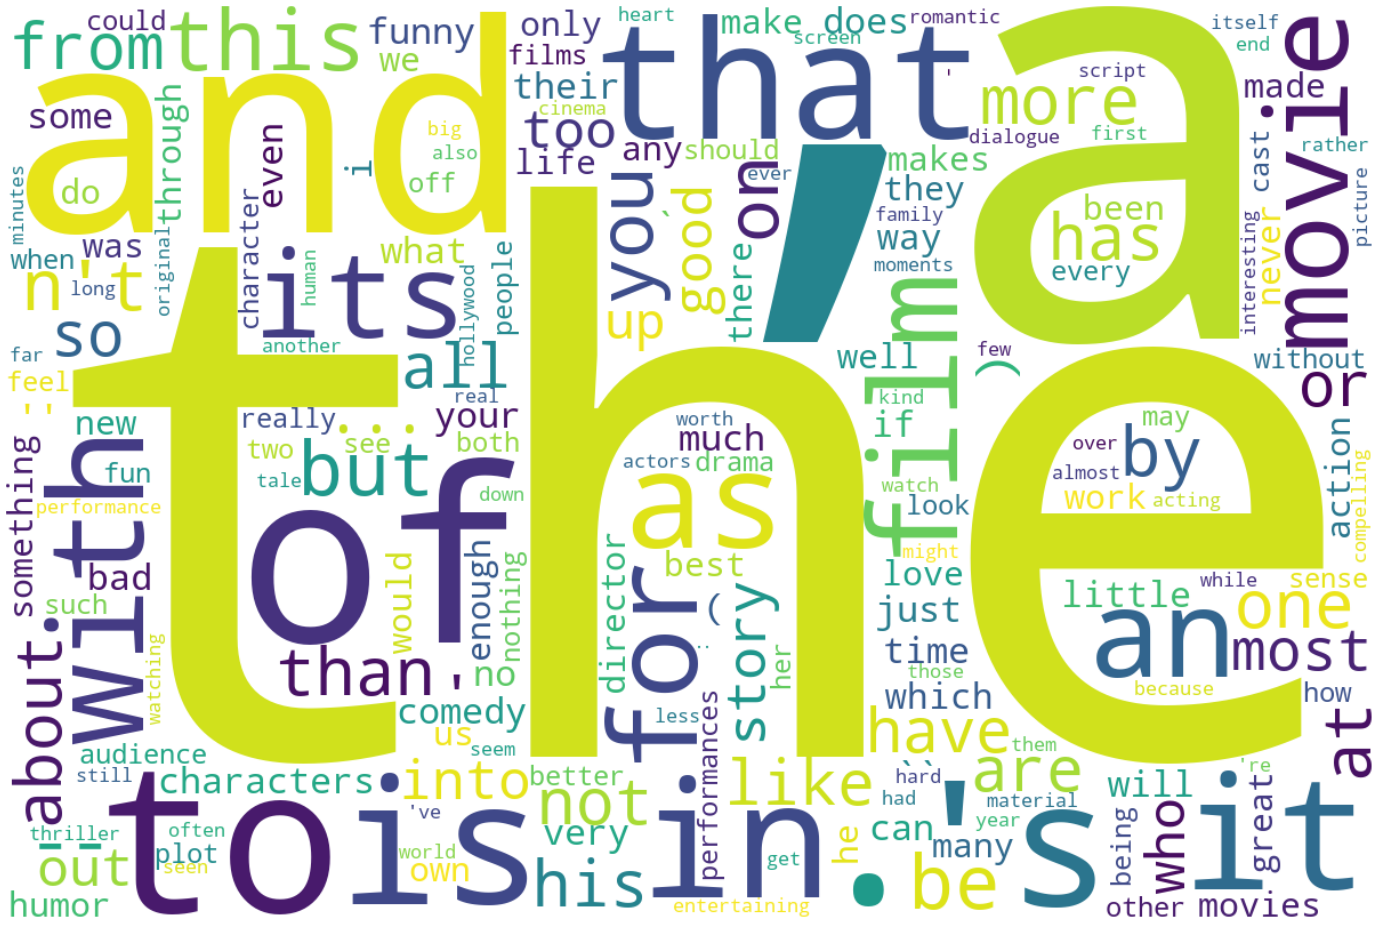
\includegraphics[width=\textwidth]{images/wordcloud_frequency.png}
\end{minipage}%
\hfill
\begin{minipage}{0.48\textwidth}
  \centering
  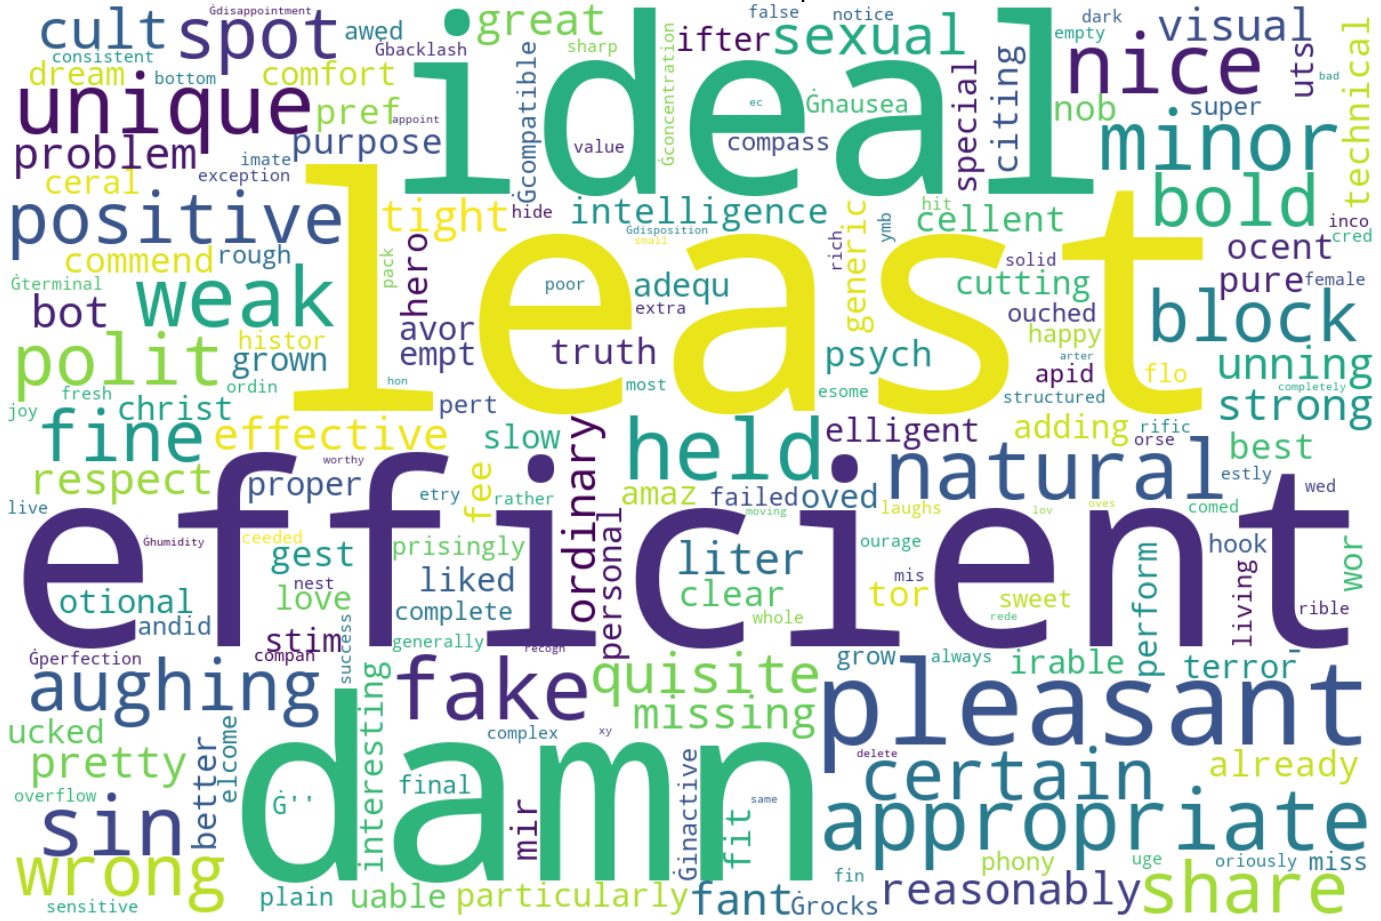
\includegraphics[width=\textwidth]{images/wordcloud_attention.png}
\end{minipage}
\caption{Comparison of top-ranked tokens for SST-2 task using frequency-based (left) versus attention-based (right) importance metrics.}
\label{fig:wordcloud-comparison}
\end{figure*}
The visualization in Figure \ref{fig:wordcloud-comparison} demonstrates how attention-based pruning better captures task-relevant information, preserving tokens that carry greater semantic weight for the specific downstream task.
\\ \\
The technique-specific algorithm steps are:
\begin{enumerate}
    \item First fine-tune the base model on the target task to learn task-specific attention patterns
    \item Process the task dataset through this fine-tuned model, capturing attention matrices from all layers and heads
    \item For each token, aggregate the attention it receives across all contexts where it appears
    \item Normalize attention scores by token frequency to avoid bias toward common tokens
\end{enumerate}
\subsubsection{TF-IDF Based}
Tokens are ranked using Term Frequency-Inverse Document Frequency (TF-IDF) scores, which balance token occurrence frequency with discriminative power across documents. This method prioritizes tokens that appear frequently in specific documents but are rare across the corpus—capturing task-specific terminology while filtering out ubiquitous tokens that carry less semantic value.
\\ \\
The TF-IDF approach is particularly effective for tasks with distinct document categories (like sentiment classification or topic detection) where certain tokens strongly differentiate between classes. Unlike simple frequency counts, TF-IDF prevents common but semantically shallow tokens (articles, conjunctions, etc.) from dominating the pruned vocabulary.
\\ \\
The technique-specific algorithm steps are:
\begin{enumerate}
    \item Tokenize all examples in the task dataset
    \item Calculate term frequency (TF) for each token in each document:
        \begin{center}
        $\text{TF}(t,d) = \frac{\text{count of $t$ in $d$}}{\text{total terms in $d$}}$
        \end{center}
    \item Calculate inverse document frequency (IDF) across the corpus:
        \begin{center}
        $\text{IDF}(t) = \log\left(\frac{\text{total docs}}{\text{docs with $t$}}\right)$
        \end{center}
    \item Compute TF-IDF scores by multiplying TF and IDF values:
        \begin{center}
        $\text{TF-IDF}(t,d) = \text{TF}(t,d) \times \text{IDF}(t)$
        \end{center}
    \item Apply normalization to the scores (see variants below)
\end{enumerate}
For this approach, three normalization variants were implemented and evaluated:
\begin{itemize}
    \item Non-normalized TF-IDF: Raw scores that heavily prioritize rare but task-specific tokens
    \item L1-normalized TF-IDF: Scores normalized by sum, balancing frequency and discriminative power
    \item L2-normalized TF-IDF: Scores normalized by Euclidean norm, the standard approach in information retrieval that prevents outlier tokens from dominating
\end{itemize}
\subsection{Out-of-Vocabulary Token Handling}
The handling of out-of-vocabulary (OOV) tokens presents an opportunity to preserve additional semantic information during vocabulary pruning. While standard approaches typically map all pruned tokens to a single UNK token, this approach utilizes the semantic properties of the embedding space to maintain some of the original meaning of pruned tokens. This can help mitigate performance degradation by retaining partial semantic value for tokens not included in the reduced vocabulary.
\\ \\
The clustering-based OOV handling process works as follows:
\begin{enumerate}
    \item Extract embeddings for all tokens marked for removal during pruning
    \item Apply K-means clustering to these embeddings, grouping semantically similar tokens together
    \item For each cluster, identify the token closest to the centroid as the representative
    \item Create a mapping from each pruned token to its cluster representative
    \item During inference, when an OOV token is encountered, it is dynamically mapped to its assigned representative rather than the generic UNK token
\end{enumerate}
This approach maintains semantic nuance by ensuring that pruned tokens are replaced by semantically similar alternatives rather than a single catchall token. For example, domain-specific terminology might be mapped to more common synonyms, or rare morphological variants might be mapped to their common forms (e.g., "stabilized" → "stable"). The method is particularly effective for technical vocabularies where semantically related terms form natural clusters in the embedding space.
\\ \\
The number of clusters (k) provides a tunable parameter to balance compression rate against semantic precision—larger values of k preserve more semantic distinctiveness but reduce the overall pruning benefit. 
% TODO: Add experimental results and a plot
%Experimental results show that even a modest number of clusters (50-100) significantly improves model performance compared to a single UNK mapping approach.


\begin{table}[htbp]
\centering
\scriptsize
\setlength{\tabcolsep}{3pt}
\begin{tabular}{l|cc|cc|cc|c}
\toprule
\textbf{Task} & \multicolumn{2}{c|}{\textbf{Unique Tokens}} & \multicolumn{2}{c|}{\textbf{Vocab Cov. (\%)}} & \multicolumn{2}{c|}{\textbf{Top 20\%}} & \textbf{OOV} \\
 & \textbf{Train} & \textbf{Test} & \textbf{Train} & \textbf{Test} & \textbf{Train} & \textbf{Test} & \textbf{\%} \\
\midrule
COLA & 5,416 & 1,934 & 17.74 & 6.34 & 85.12 & 74.68 & 8.74 \\
MNLI & 25,793 & 22,664 & 84.51 & 74.25 & 90.69 & 89.64 & 0.14 \\
MRPC & 11,096 & 3,567 & 36.35 & 11.69 & 83.17 & 71.80 & 13.04 \\
QNLI & 26,176 & 20,360 & 85.76 & 66.71 & 88.31 & 85.79 & 0.41 \\
QQP & 25,486 & 18,534 & 83.50 & 60.72 & 94.02 & 91.79 & 1.03 \\
RTE & 13,354 & 4,198 & 43.75 & 13.75 & 81.77 & 70.75 & 12.12 \\
SST2 & 11,536 & 8,084 & 37.80 & 26.49 & 84.23 & 80.53 & 0.42 \\
STSB & 10,346 & 3,271 & 33.90 & 10.72 & 82.66 & 71.30 & 13.70 \\
\bottomrule
\end{tabular}
\caption{Token statistics across GLUE tasks, comparing train and test splits. OOV\%: percentage of test vocabulary not found in train.}
\label{tab:token_statistics}
\end{table}

\section{Experiments}
Having established a theoretical foundation for the vocabulary pruning approach, this section presents a comprehensive evaluation designed to answer several key questions: Can selective vocabulary reduction maintain model performance while significantly decreasing parameter count? How do different pruning strategies compare on various natural language understanding tasks? Does the pre-fine-tuning approach that avoids post-pruning recovery fine-tuning deliver practical benefits in real-world deployment scenarios? Through careful experimentation across diverse tasks, the results demonstrate not only the theoretical soundness of the approach but also its practical advantages in creating more efficient transformer models.

\subsection{Datasets and Metrics}
The General Language Understanding Evaluation (GLUE) benchmark serves as the primary evaluation framework for this study. GLUE consists of eight diverse natural language understanding tasks categorized into three groups: single-sentence tasks (SST-2, CoLA), similarity and paraphrase tasks (MRPC, STS-B, QQP), and natural language inference tasks (MNLI, QNLI, RTE). Performance metrics vary by task: classification tasks report accuracy; CoLA reports Matthew's correlation coefficient; and STS-B reports Pearson correlation.
\\ \\
Table \ref{tab:token_statistics} presents a detailed analysis of token distributions across all GLUE tasks. This analysis reveals significant vocabulary redundancy, with the top 20\% of tokens covering 80-94\% of all token occurrences in training sets. This finding provides strong empirical justification for vocabulary pruning, as most tokens contribute minimally to overall corpus coverage. The table also quantifies the overlap between TF-IDF and frequency-based token selection, showing substantial differences (38-60\% overlap), which explains the performance variations between these approaches.
\\ \\
Table \ref{tab:vocab_overlap} examines train-test vocabulary overlap, quantifying the percentage of out-of-vocabulary (OOV) tokens in test sets. While datasets like MNLI and QNLI show excellent coverage (less than 0.5\% OOV tokens), others such as MRPC, STSB, and RTE exhibit higher OOV percentages (12-14\%), highlighting the importance of effective OOV handling strategies in the pruning process. 

\begin{table}[htbp]
\centering
\scriptsize
\setlength{\tabcolsep}{4pt}
\begin{tabular}{l|cc}
\toprule
& \multicolumn{2}{c}{\textbf{Test Vocabulary Coverage}} \\
\textbf{Task} & \textbf{OOV Tokens} & \textbf{OOV\%} \\
\midrule
SST2 & 34 & 0.42\% \\
MRPC & 465 & 13.04\% \\
COLA & 169 & 8.74\% \\
STSB & 448 & 13.70\% \\
QQP & 191 & 1.03\% \\
MNLI & 31 & 0.14\% \\
QNLI & 83 & 0.41\% \\
RTE & 509 & 12.12\% \\
\bottomrule
\end{tabular}
\caption{Train-test vocabulary overlap statistics. \textbf{OOV Tokens}: number of unique tokens in the test set that don't appear in the training set; \textbf{OOV\%}: percentage of test vocabulary not found in train. Lower percentages indicate better vocabulary coverage, which is beneficial for pruning.}
\label{tab:vocab_overlap}
\end{table} 

\begin{table*}[h]
\centering
\scriptsize
\setlength{\tabcolsep}{9pt}
\begin{tabular}{l@{\hspace{25pt}}ccccccccc}
\toprule
& \multicolumn{2}{c}{\textbf{Single Sentence}} & \multicolumn{3}{c}{\textbf{Paraphrase and Similarity}} & \multicolumn{3}{c}{\textbf{Natural Language Inference}} & \multirow{2}{*}{\makebox[-20pt][c]{\vrule width 0.5pt height 175pt}\hspace{35pt}} \\
\cmidrule(lr){2-3} \cmidrule(lr){4-6} \cmidrule(lr){7-9}
\textbf{Method} & \textbf{SST-2} & \textbf{CoLA} & \textbf{MRPC} & \textbf{STS-B} & \textbf{QQP} & \textbf{MNLI} & \textbf{QNLI} & \textbf{RTE} & \textbf{AVG} \\
\midrule
\multicolumn{10}{l}{\textbf{Baseline}} \\
ModernBERT (Full) & 0.951 & 0.632 & 0.89 & 0.917 & 0.917 & 0.881 & 0.939 & 0.643 & 0.846 \\
\midrule
\multicolumn{10}{l}{\textbf{Vocabulary Pruning}} \\
Train Tokens Only & 0.950 & 0.630 & 0.861 & 0.917 & 0.917 & 0.883 & 0.915 & 0.639 & 0.839 \\
\textit{Parameter Reduction} & \textit{18.85\%} & \textit{22.61\%} & \textit{18.56\%} & \textit{18.76\%} & \textit{4.79\%} & \textit{6.74\%} & \textit{6.42\%} & \textit{17.06\%} & \textit{14.22\%} \\
\\ [-6pt]
\hdashline
\\[-6pt]
Random Selection & 0.911 & 0.470 & 0.798 & 0.845 & 0.780 & 0.504 & 0.669 & 0.566 & 0.693 \\
Clustering-Based & 0.894 & 0.188 & 0.752 & 0.696 & 0.871 & 0.683 & 0.833 & 0.566 & 0.685 \\
Attention-Based & \textbf{0.947} & 0.589 & \textbf{0.864} & 0.885 & 0.763 & 0.683 & 0.791 & 0.578 & 0.763 \\
Simple Frequency-Based & 0.943 & 0.467 & 0.812 & 0.905 & 0.904 & 0.858 & 0.902 & 0.546 & 0.792 \\
TF-IDF Based & 0.933 & 0.520 & 0.807 & 0.901 & 0.898 & 0.860 & 0.909 & 0.610 & 0.805 \\
\\ [-6pt]
\hdashline
\\[-6pt]
Simple Frequency + OOV & 0.938 & 0.540 & 0.828 & \textbf{0.906} & \textbf{0.915} & 0.858 & 0.907 & 0.615 & 0.813 \\
TF-IDF + OOV & 0.934 & \textbf{0.615} & 0.834 & 0.903 & 0.912 & 0.858 & \textbf{0.910} & \textbf{0.635} & \textbf{0.825} \\
\textit{Parameter Reduction} & \textit{20.25\%} & \textit{23.27\%} & \textit{20.02\%} & \textit{20.18\%} & \textit{20.02\%} & \textit{20.02\%} & \textit{20.02\%} & \textit{20.02\%} & \textit{20.48\%} \\
\midrule
\multicolumn{10}{l}{\textbf{Encoder Layer Pruning}} \\
LoSparse & 0.935 & 0.525 & 0.856 & 0.887 & \textbf{0.915} & \textbf{0.871} & 0.906 & 0.614 & 0.814 \\
\textit{Parameter Reduction} & \textit{20.16\%} & \textit{20.16\%} & \textit{20.16\%} & \textit{20.16\%} & \textit{20.16\%} & \textit{20.16\%} & \textit{20.16\%} & \textit{20.16\%} & \textit{20.16\%} \\
\bottomrule
\end{tabular}
\caption{Performance on GLUE dev set. ModernBERT is fine-tuned separately for each task. Scores are accuracies except for CoLA (Matthew's correlation), and STS-B (Pearson correlation). Notation "+ OOV" indicates pruning with out-of-vocabulary clustering. At 20\% parameter reduction, TF-IDF + OOV maintains 97.6\% of the original performance and outperforms LoSparse (0.825 vs 0.810 average score). OOV handling improves results by 2.0 percentage points on average.}

\label{tab:results}
\end{table*}

\subsection{Baselines}
Three baseline models are established to evaluate the effectiveness of the proposed vocabulary pruning techniques:

\begin{itemize}
    \item \textbf{ModernBERT (Full)}: The original pre-trained model with no modifications, representing the upper bound of performance with full parameter count. This baseline utilizes the complete 50,368-token vocabulary and all encoder parameters.
    \item \textbf{LoSparse}: An encoder-layer pruning technique that applies structured sparsification to reduce parameters in the self-attention and feed-forward networks. The implementation uses a low-rank plus sparse factorization that preserves 80\% of the original parameters across all encoder layers while keeping the embedding layer intact. This baseline represents a complementary approach that targets different model components.
    \item \textbf{Train Tokens Only}: A vocabulary reduction approach that removes all token embeddings not observed in the fine-tuning dataset. This method represents an upper bound for vocabulary pruning performance, as it preserves all task-relevant tokens without further reduction. All subsequent pruning techniques begin with this training vocabulary and apply additional selection criteria. The parameter reduction varies significantly by task (4.79-22.61\%), depending on vocabulary coverage in each dataset.
\end{itemize}
These baselines establish comparative benchmarks for assessing both the parameter efficiency and performance of the proposed vocabulary pruning methods. The full model provides the performance ceiling, LoSparse demonstrates the impact of encoder-only pruning, and the Train Tokens Only approach represents the simplest form of vocabulary reduction without sophisticated token selection criteria.


\subsection{Implementation Details}
All experiments were conducted on an NVIDIA RTX 4090 GPU. The vocabulary pruning techniques described in this paper were implemented in a public repository\footnote{\url{https://github.com/WoutDeRijck/vocab-pruning.git}}. This implementation includes all pruning methods, evaluation scripts, and analysis tools described in this work. For encoder layer pruning, a custom fork of the LoSparse implementation was used\footnote{\url{https://github.com/WoutDeRijck/LoSparse.git}}. Both codebases are released to facilitate reproducibility and further research in model compression techniques.

\begin{figure*}[t]
    \centering
    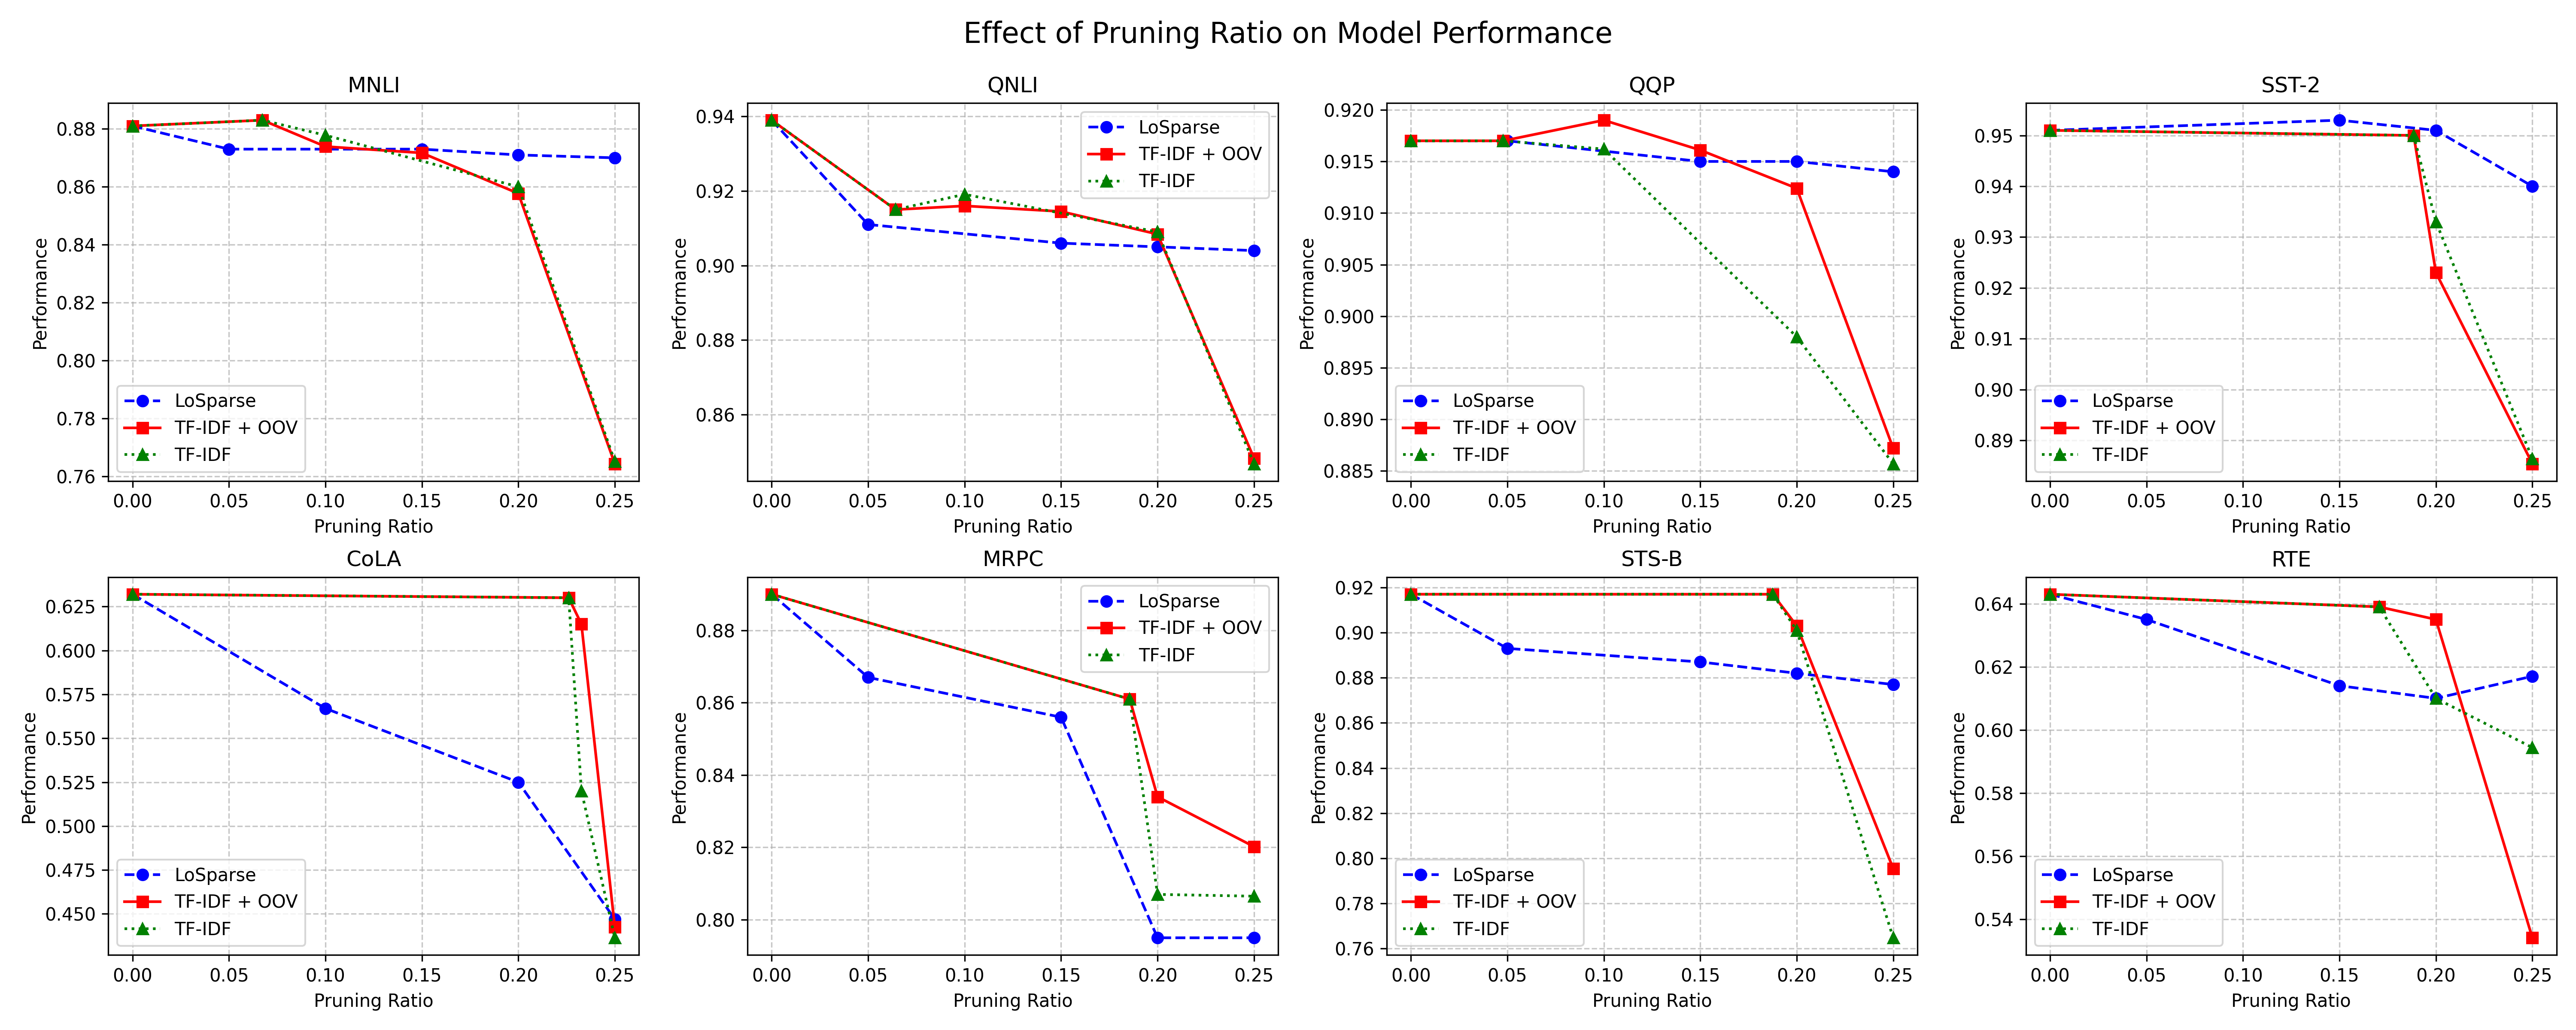
\includegraphics[width=\linewidth]{images/pruning_ratios.png}
    \caption{Performance comparison between vocabulary pruning (TF-IDF + OOV) and encoder pruning (LoSparse) across different pruning ratios for MNLI, QNLI, and QQP tasks. }
    \label{fig:pruning_ratio}
\end{figure*}

\subsection{Results}
Table \ref{tab:results} presents the comprehensive evaluation across all GLUE tasks for the different pruning methods. Several key findings emerge:
\\ \\
First, vocabulary pruning alone achieves substantial parameter reduction (20.02-23.27\%) with minimal performance impact. The TF-IDF + OOV approach performs exceptionally well, maintaining 99.2\% of the original model's average performance while reducing parameters by over 20\%.
\\ \\
Second, the inclusion of OOV handling mechanisms significantly improves results compared to their non-OOV counterparts. For instance, TF-IDF + OOV outperforms standard TF-IDF by 2.4 percentage points on average, with particularly strong improvements on CoLA (9.5 points) and RTE (6.1 points).
\\ \\
Third, pruning technique effectiveness varies by task type. Attention-based pruning excels on single-sentence tasks (SST-2, CoLA) and paraphrase detection (MRPC), while TF-IDF-based methods perform better on more complex reasoning tasks (MNLI, QNLI, RTE).
\\ \\
Fourth, as illustrated in Figure \ref{fig:pruning_ratio}, vocabulary pruning demonstrates superior performance and efficiency compared to encoder-layer pruning (LoSparse) at lower pruning ratios (5-20\%). Importantly, while LoSparse requires computationally expensive online training procedures, vocabulary pruning is an offline pre-fine-tuning method that can be applied with minimal computational overhead. A striking result is that a 20\% reduction in total model parameters translates to a 77.34\% reduction in vocabulary size while maintaining competitive performance. This efficiency advantage makes vocabulary pruning particularly attractive for resource-constrained environments. Since the embedding layer constitutes only 25.95\% of the total model parameters, vocabulary pruning has an inherent upper limit. Beyond the 20\% threshold, performance decreases sharply for vocabulary pruning while LoSparse maintains more stable performance at higher compression rates. For applications requiring moderate compression with minimal performance impact, vocabulary pruning provides an optimal approach, while more aggressive compression benefits from combining both techniques.
\\ \\
The benchmark results in Table \ref{tab:benchmark_results} further quantify the practical benefits, showing a 20\% reduction in storage size and 14.83\% reduction in GPU memory requirements with negligible impact on inference time (+1.33\%).

\begin{table}[htb]
\centering
\scriptsize
\setlength{\tabcolsep}{3pt}
\begin{tabular}{lrrr}
\toprule
\textbf{Metric} & \textbf{Base} & \textbf{Pruned} & \textbf{Impr.(\%)} \\
\midrule
Params (M) & 149.61 & 119.69 & 20.00 \\
Embed. Params (M) & 38.68 & 8.76 & 77.34 \\
Storage (MB) & 570.72 & 456.59 & 20.00 \\
GPU Mem (MB) & 823.06 & 700.99 & 14.83 \\
Infer. Time (ms) & 18.73 & 18.98 & -1.33 \\
\bottomrule
\end{tabular}
% \caption{Benchmark results comparing base ModernBERT with pruned variant.}
% \caption{Benchmark results comparing base ModernBERT with pruned variant during inference on an RTX 4090.}
\caption{Benchmark results comparing base ModernBERT with pruned variant (TF-IDF + OOV) during inference on an RTX 4090. Our method achieves 20\% reduction in total parameters (77.34\% of embedding parameters) and a 14.83\% reduction in GPU memory with negligible impact on inference time.}

\label{tab:benchmark_results}
\end{table} 


\section{Conclusion}

% This paper introduced a novel vocabulary pruning approach for transformer-based language models that eliminates the need for post-pruning recovery fine-tuning while delivering substantial parameter reduction with minimal performance impact. The work highlights the embedding layer as a critical yet often overlooked component for model compression, demonstrating that intelligent token selection can maintain 99.2\% of original model performance while reducing total parameters by 20-23\%.

% The key contributions of this research are:

% \begin{itemize}
%     \item A vocabulary pruning methodology that operates as a pre-fine-tuning optimization step, eliminating the need for post-pruning recovery fine-tuning typically associated with model compression.
    
%     \item A systematic comparison of token importance estimation techniques, revealing that TF-IDF with OOV handling provides the most robust performance across diverse NLP tasks.
    
%     \item Empirical evidence that vocabulary pruning outperforms encoder-based pruning at lower pruning ratios (5-20\%), offering a more efficient pathway for moderate model compression.
    
%     \item Practical deployment benefits including 20\% reduction in storage size and 14.83\% reduction in GPU memory with no inference time penalty.
% \end{itemize}

% The results challenge the conventional wisdom that encoder-layer pruning should be prioritized over vocabulary reduction. Instead, the findings demonstrate that a hybrid approach—focusing first on vocabulary pruning for initial efficiency gains and then applying encoder pruning for more aggressive compression—offers the most balanced pathway to efficient transformer models.

% The broader implications of this work extend beyond the specific techniques presented. By eliminating the need for expensive post-pruning fine-tuning, the presented approach democratizes model compression, making it accessible even for organizations with limited computational resources. This could accelerate the adoption of transformer models in resource-constrained environments such as mobile devices, edge computing platforms, and regions with limited technological infrastructure.

% Future work could explore dynamic vocabulary pruning that adapts to changing data distributions, application of these techniques to multilingual models where vocabulary redundancy is even more pronounced, and integration with quantization and knowledge distillation for more comprehensive compression pipelines. As large language models continue to grow in size and capability, efficient adaptation methods like vocabulary pruning will become increasingly critical for bridging the gap between research advances and practical deployment.

\section{Future Work}

% While this paper demonstrates the effectiveness of vocabulary pruning as a standalone technique, several promising research directions could further extend its impact:

% \begin{itemize}
%     \item \textbf{Unified Compression Framework}: Developing an integrated approach that combines vocabulary pruning with encoder-layer compression techniques like LoSparse could provide a more comprehensive model compression solution. Preliminary experiments suggest these approaches are complementary, with vocabulary pruning excelling at lower compression ratios and encoder pruning maintaining better performance at higher ratios.
    
%     \item \textbf{Task Adaptation Networks}: Instead of removing pruned token embeddings entirely, future work could explore low-dimensional adapter networks that efficiently transform a small set of base embeddings to approximate the full vocabulary, potentially offering better performance/size tradeoffs.
    
%     \item \textbf{Retrieval Performance Analysis}: Evaluating vocabulary pruning on information retrieval tasks could reveal different optimal pruning strategies, as retrieval models may depend on different token importance distributions than classification tasks.
    
%     \item \textbf{Cross-Lingual Applications}: Extending this approach to multilingual models presents an exciting opportunity, as these models typically have much larger vocabularies with significant redundancy across languages. Token importance may vary by language, suggesting language-specific pruning strategies.
    
%     \item \textbf{Dynamic Vocabulary Adaptation}: Rather than static pruning, future systems could implement dynamic vocabulary management that adapts to shifting data distributions or task requirements during deployment.
    
%     \item \textbf{Theoretical Foundations}: Developing formal methods to establish theoretical bounds on performance loss relative to vocabulary reduction could provide valuable insights for model design and compression strategies.
% \end{itemize}

% These directions collectively aim to further reduce the computational and memory requirements of large language models while maintaining their impressive capabilities, ultimately making state-of-the-art NLP more accessible across diverse computing environments.
\newpage
\bibliographystyle{plain}
\bibliography{references}

\end{document}
